% Three distributions with the same mean (0) and variance (1).
\documentclass[tikz,border=4pt]{standalone}
\usepackage{amsmath,amssymb}
\usepackage{pgfplots}
\pgfplotsset{compat=1.18}
\definecolor{c1}{HTML}{2F6DB5}\definecolor{c2}{HTML}{D1552B}\definecolor{c3}{HTML}{2E9E6B}
\begin{document}
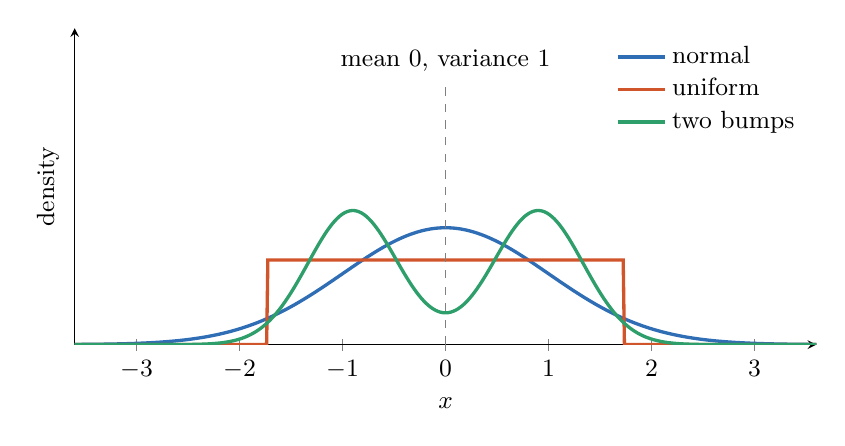
\begin{tikzpicture}
\begin{axis}[
  width=11cm, height=5.6cm, axis lines=left, domain=-3.6:3.6, samples=301,
  xmin=-3.6, xmax=3.6, ymin=0, ymax=1.08, xtick={-3,-2,-1,0,1,2,3}, ytick=\empty,
  xlabel={$x$}, ylabel={density}, every axis label/.style={font=\small},
  tick label style={font=\small},
  legend style={draw=none, fill=none, font=\small, at={(0.99,0.98)}, anchor=north east, cells={anchor=west}},
]
\addplot[c1, very thick] {exp(-x^2/2)/sqrt(2*pi)};
\addlegendentry{normal}
\addplot[c2, very thick, samples=600] {(abs(x)<=sqrt(3)) ? 1/(2*sqrt(3)) : 0};
\addlegendentry{uniform}
\addplot[c3, very thick] {0.5*(exp(-(x-0.9)^2/(2*0.19))+exp(-(x+0.9)^2/(2*0.19)))/sqrt(2*pi*0.19)};
\addlegendentry{two bumps}
\draw[dashed, gray] (axis cs:0,0) -- (axis cs:0,0.9) node[above, font=\small, black] {mean $0$, variance $1$};
\end{axis}
\end{tikzpicture}
\end{document}
